
\hyphenpenalty = 10000
\documentclass{article}




\usepackage[nonatbib, final]{neurips_2023}








\usepackage[utf8]{inputenc} %
\usepackage[T1]{fontenc}    %
\usepackage{aligned-overset}
\usepackage{amsthm}
\usepackage{amsmath}
\usepackage{amssymb}
\usepackage{comment}
\usepackage{array}
\usepackage[hidelinks,bookmarksnumbered]{hyperref}       %
\usepackage[capitalize]{cleveref}
\usepackage{url}            %
\usepackage{booktabs}       %
\usepackage{amsfonts}       %
\usepackage{nicefrac}       %
\usepackage{microtype}      %
\usepackage{xcolor}         %
\usepackage{bbm}
\usepackage{tikz}
\usepackage{pgfplots}
\pgfplotsset{compat=1.18}
\usetikzlibrary{positioning}
\usetikzlibrary{arrows.meta}
\usetikzlibrary{calc}
\usepackage{subcaption}
\usepackage{soul}
\usepackage[style = numeric, url = true, giveninits=true, eprint = false, sortcites=true,backend = biber, maxbibnames=99]{biblatex}
\addbibresource{references.bib}
\AtBeginBibliography{\small}
\AtEveryBibitem{\clearlist{language}}
\AtEveryBibitem{\clearfield{issn}}
\AtEveryCitekey{\clearfield{issn}}
\DeclareBibliographyCategory{needsurl}
\renewbibmacro*{url+urldate}{%
  \ifcategory{needsurl}
    {\printfield{url}%
     \iffieldundef{urlyear}
       {}
       {\setunit*{\addspace}%
        \printurldate}}
    {}}
\newcommand{\entryneedsurl}[1]{\addtocategory{needsurl}{#1}}
\entryneedsurl{NIPS2017_3f5ee243}
\entryneedsurl{yarotsky_phase_2021}
\entryneedsurl{arjovsky_unitary_2016}

\usepackage{todonotes}
\let \eps \varepsilon
\theoremstyle{plain} 
\newtheorem{theorem}{Theorem}[section]
\newtheorem{corollary}[theorem]{Corollary}
\newtheorem{lemma}[theorem]{Lemma}
\newtheorem{proposition}[theorem]{Proposition}
\newtheorem{Folg}[theorem]{Consequence}
\newtheorem{Verm}[theorem]{Conjecture}
\newtheorem{Probl}[theorem]{Problem}


\theoremstyle{definition} %
\newtheorem{definition}[theorem]{Definition}
\newtheorem{Bsp}[theorem]{Example}
\newtheorem{Bem}[theorem]{Remark}
\newtheorem{Alg}[theorem]{Algorithm}

\theoremstyle{remark} %
\newtheorem{remark}[theorem]{Remark}
\newtheorem{myproof}[theorem]{Proof}

\crefname{theorem}{theorem}{theorems}
\crefname{Prop}{Proposition}{Propositions}
\crefname{Lem}{Lemma}{Lemmas}
\crefname{Kor}{Corollary}{Corollaries}
\crefname{Bem}{Remark}{Remarks}
\crefname{Bsp}{Example}{Examples}
\crefname{Def}{Definition}{Definitions}
\crefname{Alg}{Algorithm}{Algorithms}

\numberwithin{equation}{section}

\newcolumntype{P}[1]{>{\centering\arraybackslash}m{#1}}

\newcommand{\defeq}{\mathrel{\mathop:}=}    
\newcommand{\CC}{\mathbb{C}}
\newcommand{\RR}{\mathbb{R}}
\newcommand{\NN}{\mathbb{N}}
\newcommand{\QQ}{\mathbb{Q}}
\newcommand{\Z}{\mathbb{Z}}
\newcommand{\ZZ}{\mathbb{Z}}
\newcommand{\wirt}{\partial_{\mathrm{wirt}}}
\newcommand{\wirtq}{\overline{\partial}_{\mathrm{wirt}}}
\newcommand{\m}{\textbf{m}}
\newcommand{\elll}{\boldsymbol{\ell}}
\newcommand{\PP}{\mathcal{P}}
\newcommand{\pp}{\textbf{p}}
\newcommand{\qq}{\textbf{q}}
\newcommand{\rr}{\textbf{r}}
\newcommand{\kk}{\textbf{k}}
\newcommand{\modrelu}{\sigma_{\mathrm{modReLU}, b}}
\newcommand*{\fres}[2]{ {\left.\kern-\nulldelimiterspace #1 \vphantom{\big|} \right|_{\kern-1pt #2} }}
\newcommand{\defequiv}{\mathrel{\mathop:}\Leftrightarrow}
\newcommand{\norel}{\mathrel{\phantom{=}}}       
\newcommand{\aalpha}{\boldsymbol{\alpha}}
\newcommand{\nuu}{\boldsymbol{\nu}}
\newcommand{\paul}{\textcolor{red}}
\DeclareMathOperator{\RE}{Re}
\DeclareMathOperator{\IM}{Im}
\DeclareMathOperator{\spann}{span}
\DeclareMathOperator{\supp}{supp}

\let\emptyset\varnothing


\DeclareMathOperator{\card}{card}


\binoppenalty=\maxdimen
\relpenalty=\maxdimen
\overfullrule=1mm

\title{Optimal approximation \\ using complex-valued neural networks}




\author{
  Paul Geuchen \\
  MIDS, \\ KU Eichstätt-Ingolstadt,\\
  Auf der Schanz 49, \\85049 Ingolstadt, Germany \\
  \texttt{paul.geuchen@ku.de} \\
   \And
  Felix Voigtlaender\\
  MIDS, \\ KU Eichstätt-Ingolstadt, \\
  Auf der Schanz 49, \\85049 Ingolstadt, Germany \\
   \texttt{felix.voigtlaender@ku.de} \\
}


\begin{document}


\maketitle


\begin{abstract}
  Complex-valued neural networks (CVNNs) have recently shown promising empirical success, for instance for increasing the stability of recurrent neural networks and for improving the performance in tasks with complex-valued inputs, such as in MRI fingerprinting. While the overwhelming success of Deep Learning in the real-valued case is supported by a growing mathematical foundation, such a foundation is still largely lacking in the complex-valued case.
  We thus analyze the expressivity of CVNNs by studying their approximation properties.
  Our results yield the first quantitative approximation bounds for CVNNs that apply
  to a wide class of activation functions including the popular modReLU and complex cardioid activation functions.
  Precisely, our results apply to any activation function that is smooth but not polyharmonic
  on some non-empty open set; this is the natural generalization of the class of
  smooth and non-polynomial activation functions to the complex setting.
  Our main result shows that the error for the approximation of $C^k$-functions
  scales as $m^{-k/(2n)}$ for $m \to \infty$ where $m$ is the number of neurons,
  $k$ the smoothness of the target function and $n$ is the (complex) input dimension.
  Under a natural continuity assumption, we show that this rate is optimal;
  we further discuss the optimality when dropping this assumption.
  Moreover, we prove that the problem of approximating $C^k$-functions
  using continuous approximation methods unavoidably suffers from the curse of dimensionality.
\end{abstract}


\section{Introduction}


Deep Learning currently predominantly relies on real-valued neural networks,
which have led to breakthroughs in fields like image classification or speech recognition
\cite{6638947, krizhevsky_imagenet_2017,NIPS2017_3f5ee243}.
However, recent work has uncovered several application areas in which
the use of complex-valued neural networks (CVNNs) leads to better results
than the use of their real-valued counterparts.
These application areas mainly include tasks where complex numbers inherently occur as inputs
of a machine learning model such as Magnetic Resonance Imaging (MRI)
\cite{virtue_better_2017,cole2021analysis,el2020deep}
and Polarimetric Synthetic Aperture Radar (PolSAR) Imaging
\cite{8039431,barrachina2023comparison,barrachina2021complex}.
Moreover, CVNNs have been used to improve the stability of recurrent neural networks
\cite{arjovsky_unitary_2016} and have been successfully applied in various other fields
\cite{8356260,qu2023entanglement}.
The mathematical theory of these complex-valued neural networks, however,
is still in its infancy.
There is therefore a great interest in studying CVNNs
and in particular in uncovering the differences and commonalities between CVNNs
and their real-valued counterparts. 
A prominent example highlighting the unexpected differences between both network classes
is the \emph{universal approximation theorem} for neural networks,
whose most general real-valued version was proven in 1993 \cite{leshno_multilayer_1993}
(with a more restricted version appearing earlier \cite{cybenko_approximation_1989})
and which was recently generalized to the case of CVNNs \cite{voigtlaender_universal_2022}.
The two theorems describe necessary and sufficient conditions on an activation function
which guarantee that arbitrarily wide neural networks of a fixed depth can approximate any
continuous function on any compact set arbitrarily well (with respect to the uniform norm).
Already here it was shown that complex-valued networks behave significantly different
from real-valued networks: While real-valued networks are universal if and only if
the activation function is non-polynomial, complex-valued networks with a single hidden layer
are universal if and only if the activation function is non-polyharmonic (see below for a definition).
Furthermore, there exist continuous activation functions for which deep CVNNs are universal
but shallow CVNNs are not, whereas the same cannot happen for real-valued neural networks.
This example shows that it is highly relevant to study the properties of CVNNs
and to examine which of the fundamental properties of real-valued networks extend to complex-valued networks.
\renewcommand{\arraystretch}{1.5}

\begin{table}
\centering
\begin{tabular}{P{0.2\linewidth}|P{0.2\linewidth}|P{0.2\linewidth}|P{0.2\linewidth}} 
&Condition on activation function & Continuity of weight selection & Approximation Error \\ \hline
\Cref{main_2}& smooth \& non-polyharmonic&possible& $\mathcal{O}(m^{-k/(2n)})$ \\ \hline
Consequence of \Cref{thm:opti_conti}& continuous & assumed & $\Omega(m^{-k/(2n)})$ \\ \hline
\Cref{main_4}& very special activation function & not assumed & $\mathcal{O}(m^{-k/(2n-1)})$ \\ \hline
\Cref{main_5}& \rule{0pt}{0.65cm}$\displaystyle\frac{1}{1 + e^{-\mathrm{Re}(z)}}$ & not assumed & $\widetilde{\Omega}(m^{-k/(2n)})$
\end{tabular}
\vspace{0.3cm}
\caption{Overview of the proven approximation bounds.
$k$ is the regularity of the approximated functions (which are assumed to be $C^k$),
$n$ the (complex) input dimension and $m$ the number of neurons in the hidden layer of the network.
The notation $\widetilde{\Omega}$ is similar to $\Omega$, but ignoring log factors.}
\label{tab:overview}
\end{table}
\raggedbottom


Essentially the only existing \emph{quantitative} result regarding
the approximation-theoretical properties of CVNNs is \cite{caragea_quantitative_2022},
which provides results for approximating $C^k$-functions by \emph{deep} CVNNs
using the modReLU activation function.
However, for real-valued NNs it is known that already \emph{shallow} NNs can approximate
$C^k$-functions at the optimal rate.
Precisely, Mhaskar showed in \cite{mhaskar_neural_1996} that one can approximate $C^k$-functions
on $[-1,1]^n$ with an error of order $m^{-k/n}$ as $m \to \infty$,
where $m$ is the number of neurons in the hidden layer.
Here he assumed that the activation function is smooth on an open interval and that at some point
of this interval no derivative vanishes.
This is equivalent to the activation function being smooth and non-polynomial on that interval,
cf.\ \cite[p.~53]{donoghue_distributions_1969}.

The present paper shows that a comparable result holds in the setting of complex-valued networks,
by proving that one can approximate every function in $C^k \left( \Omega_n; \CC \right)$
(where differentiability is understood in the sense of real variables)
with an error of the order $m^{-k/(2n)}$ (as $m \to \infty$) using shallow
complex-valued neural networks with $m$ neurons in the hidden layer.
Here we define the cube $\Omega_n \defeq [-1,1]^n + i [-1,1]^n$.
The result holds whenever the activation function $\phi: \CC \to \CC$ is smooth and non-polyharmonic
on some non-empty open set.
This is a very natural condition, since for polyharmonic activation functions there exist
$C^k$-functions that cannot be approximated at all below some error threshold
using shallow neural networks with this activation function \cite{voigtlaender_universal_2022}.

Furthermore, the present paper studies in how far the approximation order of $m^{-k/(2n)}$
is \emph{optimal}, meaning that an order of $m^{-(k/2n) - \alpha}$ (where $\alpha > 0$)
cannot be achieved.
Here it turns out that the derived order of approximation is indeed optimal
(even in the class of CVNNs with possibly more than one hidden layer)
in the setting that the weight selection is \emph{continuous},
meaning that the map that assigns to a function $f \in C^k \left( \Omega_n;\CC\right)$
the weights of the approximating network is continuous with respect to some norm on $C^k (\Omega_n ; \CC)$.
This continuity assumption is natural since typical learning algorithms
such as (stochastic) gradient descent use samples $f(x_j)$ of the target function
and then apply continuous operations to them to update the network weights. 

We investigate this optimality result further by dropping the continuity assumption
and constructing two special smooth and non-polyharmonic activation functions
with the first one having the property that the order of approximation can indeed be strictly improved
via a \emph{discontinuous} selection of the related weights.
For the second activation function we show that the order of $m^{-k/(2n)}$ \emph{cannot} be improved,
even if one allows a discontinuous weight selection.
This in particular shows that in the given generality of arbitrary smooth,
non-polyharmonic activation functions, the upper bound $\mathcal{O}\left(m^{-k/(2n)}\right)$
cannot be improved, even for a possibly discontinuous choice of the weights.
An overview of the approximation bounds proven in this paper can be found in \Cref{tab:overview}.

Moreover, we analyze the \emph{tractability} (in terms of the input dimension $n$)
of the considered problem of approximating $C^k$-functions using neural networks.
\Cref{thm:intrac} shows that one necessarily needs a number of parameters \emph{exponential}
in $n$ to obtain a non-trivial approximation error.
To the best of our knowledge, \Cref{thm:intrac} is the first result showing that the problem
of approximating $C^k$-functions using continuous approximation methods is intractable
(in terms of the input dimension $n$).

\subsection{Related Work}
\textbf{Real-valued neural networks.}
By now, the approximation properties of real-valued neural networks are quite well-studied
(cf.\ \cite{leshno_multilayer_1993,yarotsky_error_2017,barron1993universal,CiCP-28-1768,SIEGEL2020313,mhaskar_neural_1996,yarotsky_phase_2021} and the references therein).
We here only discuss a few papers that are most closely related to the present work.

In \cite{mhaskar_neural_1996}, Mhaskar analyzes the rate of approximation of
shallow real-valued neural networks for target functions of regularity $C^k$.
Our results can be seen as the generalization of \cite{mhaskar_neural_1996} to the complex setting.
Our proofs rely on several techniques from \cite{mhaskar_neural_1996};
however, significant modifications are required to make the proofs work for general smooth non-polyharmonic functions. 

One of the first papers to observe that neural networks with general (smooth) activation function
can be surprisingly expressive is \cite{MAIOROV199981} where it was shown that a neural network
of \emph{constant size} can be universal.
One of the activation functions in \Cref{sec:optimality} is based on a similar idea.

The importance of distinguishing between continuous and discontinuous weight selection
(which in our setting is discussed in \Cref{sec:optimality}) was observed for ReLU-networks in \cite{yarotsky_phase_2021}. 

The paper \cite{KAINEN199947} shows that neural network approximation is \emph{not} continuous in the following sense:
The best approximating neural network $\Phi(f)$ of a given size does not depend continuously on $f \in C^k$.
This result, however, is not in conflict with our results:
We want to assign to any $C^k$-function $f$ a network $\widetilde{\Phi}(f)$ that approximates $f$
below the error threshold $m^{-k/(2n)}$.
The network $\widetilde{\Phi}(f)$, however, does \emph{not} have to coincide with the best approximating network $\Phi(f)$.

\textbf{Complex-valued neural networks.}
 When it comes to general literature about mathematical properties of complex-valued neural networks,
 surprisingly little work can be found.
 The \emph{Universal Approximation Theorem for Complex-Valued Neural Networks} \cite{voigtlaender_universal_2022}
 has already been mentioned above.
 In particular, it has been shown that shallow CVNNs are universal if and only if the activation function
 $\phi$ is not polyharmonic.
 Thus, the condition assumed in the present paper (that $\phi$ should be smooth, but not polyharmonic)
 is quite natural.

Regarding \emph{quantitative} approximation results for CVNNs, the only existing work
of which we are aware is \cite{caragea_quantitative_2022},
analyzing the approximation capabilities of \emph{deep} CVNNs where the modReLU is used as activation function.
Since the modReLU satisfies our condition regarding the activation function,
the present work can be seen as an improvement to \cite{caragea_quantitative_2022}.
Precisely, (i) we consider general activation functions, including but not limited to the modReLU,
(ii) we improve the order of approximation by a log factor,
and (iii) we show that this order of approximation can be achieved using shallow networks instead of the deep networks used in \cite{caragea_quantitative_2022}.
We stress that our proof techniques differ significantly from the ones applied in \cite{caragea_quantitative_2022}:
The arguments in \cite{caragea_quantitative_2022} take their main ideas from \cite{yarotsky_error_2017}
making heavy use of the specific definition of the modReLU.
In contrast, since we consider quite general activation functions, we necessarily follow
a much more general approach following the ideas from \cite{mhaskar_neural_1996}.

\section{Preliminaries} \label{sec:prelim}

\textbf{Shallow complex-valued neural networks.} In this paper we mainly consider so-called shallow complex-valued neural networks, meaning complex-valued neural networks with a single hidden layer. Precisely, we consider functions of the form
\begin{equation*}
    \CC^n \ni z \mapsto \sum_{j=1}^{m} \sigma_j \phi\left(\rho_j^T \cdot z + \eta_j\right) \in \CC,
\end{equation*}
with $\rho_1, ..., \rho_{m} \in \CC^{n}$, $\sigma_1, ..., \sigma_{m}, \eta_1,..., \eta_{m} \in \CC$ and an \emph{activation function} $\phi:\CC \to \CC$. Here, $m \in \NN$ denotes the number of neurons of the network and we write $v^T$ for the transpose of a vector $v$.

To simplify the formulation of the results, we introduce the following notation: We write $\mathcal{F}^{\phi}_{n,m}$ for the set of \emph{first layers} of shallow complex-valued neural networks with activation function $\phi$, with $n$ input neurons and $m$ hidden neurons, meaning
\begin{equation*}
  \mathcal{F}^{\phi}_{n,m}
  \defeq \left\{
           z \mapsto \left(\phi\left(\rho_j^T \cdot z + \eta_j\right)\right)_{j=1}^m : \ \rho_j \in \CC^n, \ \eta_j \in \CC
         \right\}
  \subseteq \left\{ F: \CC^n \to \CC^m\right\}.
\end{equation*}
Hence, each shallow CVNN can be written as $\sigma^T \Phi$ with $\sigma \in \CC^m$ and $\Phi \in \mathcal{F}^{\phi}_{n,m}$;
see \Cref{fig:cvnn} for a graphical representation of a shallow CVNN.

\begin{figure}[t]
\centering
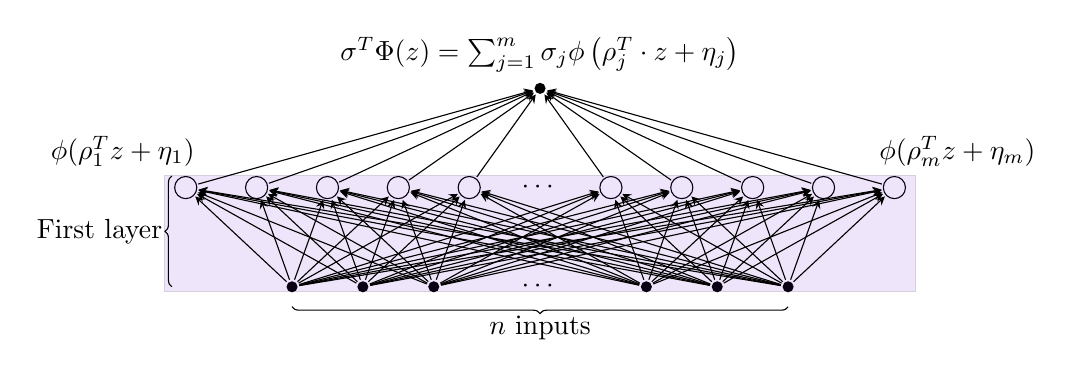
\begin{tikzpicture}[x=0.9cm,y=0.63cm,>=stealth,neuron/.style={circle,draw=black,inner sep=0pt,minimum size=8pt},
transition/.style={circle,fill=black,inner sep=0pt,minimum size=4pt},
pre/.style={->, shorten >=0.5pt,shorten <=0.5pt},
post/.style={->, shorten >=0.5pt,shorten <=0.5pt},
peri/.style={->, shorten >=0.5pt,shorten <=0.5pt}]

\node[transition] (init1) at (1,-3){};
\node[transition] (init2) at (2,-3){};
\node[transition] (init3) at (3,-3){};
\node[transition] (init4) at (6,-3){};
\node[transition] (init5) at (7,-3){};
\node[transition] (init6) at (8,-3){};
\node[neuron,label={[xshift=-0.8cm, yshift=0cm]$\phi(\rho_1^T z + \eta_1)$}] (hidden1) at (-0.5,-1){};
\node[neuron] (hidden2) at (0.5,-1){};
\node[neuron] (hidden3) at (1.5,-1){};
\node[neuron] (hidden4) at (2.5,-1){};
\node[neuron] (hidden5) at (3.5,-1){};
\node[neuron] (hidden7) at (5.5,-1){};
\node[neuron] (hidden8) at (6.5,-1){};
\node[neuron] (hidden9) at (7.5,-1){};
\node[neuron] (hidden10) at (8.5,-1){};
\node[neuron,label={[xshift=0.8cm, yshift=0cm]$\phi(\rho_m^T z + \eta_m)$}] (hidden11) at (9.5,-1){};
\node[transition, label=above:{$\sigma^T \Phi(z) = \sum_{j=1}^{m} \sigma_j \phi\left(\rho_j^T \cdot z + \eta_j\right)$}] (out) at (4.5,1){};

\definecolor{mycolor}{RGB}{102,0,204}
\draw[fill = mycolor, opacity = 0.1](-0.8,-3.1) rectangle (9.8, -0.75) ;

\draw ($(init3)!0.5!(init4)$) node{$\cdots$};
\draw ($(hidden5)!0.5!(hidden7)$) node{$\cdots$};

\draw[pre](init1)--(hidden1);
\draw[pre](init1)--(hidden2);
\draw[pre](init1)--(hidden3);
\draw[pre](init1)--(hidden4);
\draw[pre](init1)--(hidden5);
\draw[pre](init1)--(hidden7);
\draw[pre](init1)--(hidden8);
\draw[pre](init1)--(hidden9);
\draw[pre](init1)--(hidden10);
\draw[pre](init1)--(hidden11);

\draw[pre](init2)--(hidden1);
\draw[pre](init2)--(hidden2);
\draw[pre](init2)--(hidden3);
\draw[pre](init2)--(hidden4);
\draw[pre](init2)--(hidden5);
\draw[pre](init2)--(hidden7);
\draw[pre](init2)--(hidden8);
\draw[pre](init2)--(hidden9);
\draw[pre](init2)--(hidden10);
\draw[pre](init2)--(hidden11);

\draw[pre](init3)--(hidden1);
\draw[pre](init3)--(hidden2);
\draw[pre](init3)--(hidden3);
\draw[pre](init3)--(hidden4);
\draw[pre](init3)--(hidden5);
\draw[pre](init3)--(hidden7);
\draw[pre](init3)--(hidden8);
\draw[pre](init3)--(hidden9);
\draw[pre](init3)--(hidden10);
\draw[pre](init3)--(hidden11);

\draw[pre](init4)--(hidden1);
\draw[pre](init4)--(hidden2);
\draw[pre](init4)--(hidden3);
\draw[pre](init4)--(hidden4);
\draw[pre](init4)--(hidden5);
\draw[pre](init4)--(hidden7);
\draw[pre](init4)--(hidden8);
\draw[pre](init4)--(hidden9);
\draw[pre](init4)--(hidden10);
\draw[pre](init4)--(hidden11);

\draw[pre](init5)--(hidden1);
\draw[pre](init5)--(hidden2);
\draw[pre](init5)--(hidden3);
\draw[pre](init5)--(hidden4);
\draw[pre](init5)--(hidden5);
\draw[pre](init5)--(hidden7);
\draw[pre](init5)--(hidden8);
\draw[pre](init5)--(hidden9);
\draw[pre](init5)--(hidden10);
\draw[pre](init5)--(hidden11);

\draw[pre](init6)--(hidden1);
\draw[pre](init6)--(hidden2);
\draw[pre](init6)--(hidden3);
\draw[pre](init6)--(hidden4);
\draw[pre](init6)--(hidden5);
\draw[pre](init6)--(hidden7);
\draw[pre](init6)--(hidden8);
\draw[pre](init6)--(hidden9);
\draw[pre](init6)--(hidden10);
\draw[pre](init6)--(hidden11);

\draw[post](hidden1)--(out);
\draw[post](hidden2)--(out);
\draw[post](hidden3)--(out);
\draw[post](hidden4)--(out);
\draw[post](hidden5)--(out);
\draw[post](hidden7)--(out);
\draw[post](hidden8)--(out);
\draw[post](hidden9)--(out);
\draw[post](hidden10)--(out);
\draw[post](hidden11)--(out);

 \draw [decoration={brace,raise=5pt,mirror},decorate] (init1.south) -- (init6.south) node [below=5pt,pos=0.5] {$n$ inputs};
  \draw [decoration={brace,raise=5pt},decorate] (-0.5,-3) -- (hidden1.north) node [left=5pt,pos=0.5] {First layer};
\end{tikzpicture}


\caption{Graphical representation of a shallow neural network.
Input and output neurons are depicted as dots, hidden neurons are depicted as circles.
The term \emph{first layer} describes the transformation from the input to the hidden neurons,
including the application of the activation function.}
\label{fig:cvnn}
\end{figure}

\textbf{Approximation.} The paper aims to analyze the approximation of $C^k$-functions on the complex cube
\begin{equation*}
\Omega_n \defeq [-1,1]^n + i [-1,1]^n
\end{equation*}
using shallow CVNNs. Here, we say that a function $f: \Omega_n \to \CC$ is in $C^k(\Omega_n; \CC)$
if and only if $f$ is $k$ times continuously differentiable on $\Omega_n$,
where the derivative is to be understood in the sense of real variables, i.e.,
in the sense of interpreting $f$ as a function $[-1,1]^{2n} \to \RR^2$ and taking usual real derivatives.
We further define the \emph{$C^k$-norm} of a function $f \in C^k(\Omega_n; \CC)$ as
\begin{equation}\label{eq:ckdef}
  \Vert f \Vert_{C^k(\Omega_n; \CC)}
  \defeq \underset{\vert \kk \vert \leq k}{\underset{\kk \in \NN_0^{2n}}{\sup}} \Vert \partial^\kk f\Vert_{L^\infty(\Omega_n; \CC)} ,
  \qquad\text{where}\qquad
  \Vert g \Vert_{L^\infty(\Omega_n; \CC)} \defeq \sup_{z \in \Omega_n} \vert g(z) \vert
\end{equation}
for any function $g:\Omega_n \to \CC$. Note that we write $\NN = \{1,2,3,...\}$ and $\NN_0 = \{0\} \cup \NN$. Using the previously introduced notation, we thus seek to bound the worst-case approximation error, i.e.,
\begin{equation*}
  \underset{\Vert f \Vert_{C^k(\Omega_n; \CC)} \leq 1}{\sup_{f \in C^k(\Omega_n ; \CC)}} \ \
    \underset{\sigma \in \CC^m}{\inf_{\Phi \in \mathcal{F}^\phi_{n,m}}}
      \Vert f - \sigma^T \Phi \Vert_{L^\infty(\Omega_n ; \CC)}.
\end{equation*}

\textbf{Wirtinger calculus and polyharmonic functions.} For a function $f: \CC \to \CC$
which is differentiable in the sense of real variables at a point $z_0 \in \CC$
we define its \emph{Wirtinger derivatives} at $z_0$ as
\begin{equation*}
  \wirt f (z_0)
  \defeq \frac{1}{2} \left(\frac{\partial f}{\partial x}(z_0) - i \cdot \frac{\partial f}{\partial y }(z_0)\right)
  \quad \text{and} \quad
  \wirtq f (z_0)
  \defeq \frac{1}{2} \left(\frac{\partial f}{\partial x}(z_0) + i \cdot \frac{\partial f}{\partial y }(z_0)\right).
\end{equation*}
Here, $\frac{\partial}{\partial x}$ and $\frac{\partial}{ \partial y}$ denote the usual partial derivatives in the sense of real variables.
We extend this definition to multivariate functions defined on open subsets of $\CC^n$ by considering \emph{coordinatewise} Wirtinger derivatives. 

A function $f:U \to \CC$, where $U \subseteq \CC$ is an open set, is called \emph{smooth}
if it is differentiable arbitrarily many times (in the sense of real variables).
We write $f \in C^\infty(U;\CC)$ in that case. Moreover, $f$ is called \emph{polyharmonic} (on $U$)
if it is smooth and if there exists $m \in \NN_0$ satisfying
\begin{equation*}
  \Delta^m f \equiv 0 \quad \text{on} \ U.
\end{equation*}
Here, $\Delta \defeq \frac{\partial^2}{\partial x^2} + \frac{\partial^2}{\partial y^2} = 4 \wirt \wirtq$ denotes the usual Laplace-Operator.

The following \Cref{prop:nonpoly} describes a property of non-polyharmonic functions which is crucial for proving the approximation results of this paper.
\begin{proposition} \label{prop:nonpoly}
Let $\emptyset \neq U \subseteq \CC$ be an open set and let $\phi \in C^\infty(U; \CC)$ be non-polyharmonic. Then for every $M \in \NN_0$ there exists a point $z_M \in U$ satisfying
\begin{equation*}
\wirt^m \wirtq^\ell \phi (z_M) \neq 0 \quad \textrm{for} \ \textrm{all}\  m,\ell \in \NN_0 \ \textrm{with} \ m,\ell\leq M.
\end{equation*} 
\end{proposition}
The proof of \Cref{prop:nonpoly} is an application of the Baire category theorem; see \Cref{admissibility_reordered}.

\textbf{Important complex activation functions.}
We briefly discuss in how far two commonly used complex activation functions satisfy our assumptions:
The \emph{modReLU} proposed in \cite{arjovsky_unitary_2016} and the \emph{complex cardioid}
used in \cite{virtue_better_2017} for MRI fingerprinting where the performance
could be significantly improved using complex-valued neural networks.
The modReLU is defined as
\begin{equation*}
 \modrelu: \quad
 \CC \to \CC, \quad
 \modrelu(z)
 \defeq \begin{cases}
          (\vert z \vert + b)\frac{z}{\vert z \vert},& \mathrm{if} \ \vert z \vert + b \geq 0, \\
          0,& \text{otherwise,}
        \end{cases}
\end{equation*}
where $b<0$ is a fixed  parameter.
The complex cardioid is defined as
\begin{equation*}
    \card: \quad
    \CC \to \CC, \quad
    \card(z) \defeq  \frac{1}{2}(1+\mathrm{cos}(\sphericalangle z ))z.
\end{equation*}
Here, $\sphericalangle z = \theta \in \RR$ denotes the polar angle of a complex number $z = re^{i\theta}$,
where we define $\sphericalangle 0 := 0$; see \Cref{fig:abs} for plots of the absolute value of the two functions.

Both functions are smooth and non-polyharmonic on a non-empty open subset of $\CC$,
which is proven in \Cref{concrete_activation_functions_reordered}.
Furthermore, they are both continuous on $\CC$.
Therefore, our approximation bounds established in \Cref{main_1,main_2} in particular apply to those two functions.
    

\begin{figure} [t]
\centering
\begin{subfigure}{0.48\textwidth}
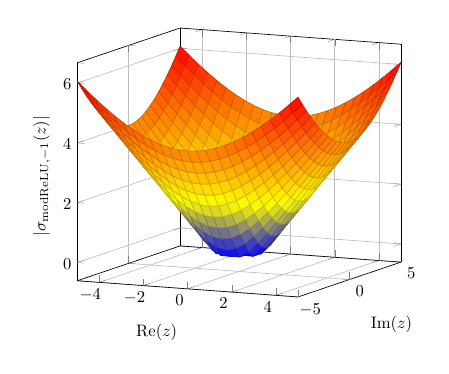
\begin{tikzpicture} [scale = 0.6]
\begin{axis}[grid = both, xlabel = $\mathrm{Re}(z)$, ylabel = $\mathrm{Im}(z)$, zlabel = $\vert \sigma_{\mathrm{modReLU}, -1} (z)\vert$,  restrict z to domain*=0:10, view={25}{10}]
\addplot3[
    surf,
]
{sqrt(x^2 + y^2) - 1};
\end{axis}
\end{tikzpicture}
\end{subfigure}
\begin{subfigure}{0.48\textwidth}
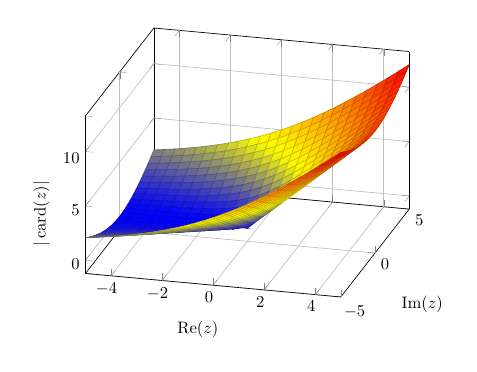
\begin{tikzpicture}[scale = 0.6]
\begin{axis}[grid = both, xlabel = $\mathrm{Re}(z)$, ylabel = $\mathrm{Im}(z)$, zlabel = $\vert \card (z)\vert$, view={15}{30}]
\addplot3[
    surf,
]
{0.5(sqrt(x^2 + y^2) + x)};
\end{axis}
\end{tikzpicture}
\end{subfigure}


\caption{Absolute value of the activation functions $\sigma_{\mathrm{modReLU}, -1}$ (left) and $\card$ (right).}
\label{fig:abs}
\end{figure}

\section{Main results} \label{sec:main}

In this section we state the main results of this paper and provide proof sketches for them.
Detailed proofs of the two statements can be found in \Cref{approx_polynomials_reordered,ck_functions_reordered}. 

First we show in \Cref{main_1} that it is possible to approximate any complex polynomial
in $z$ and $\overline{z}$ arbitrarily well using shallow CVNNs with the size of the networks
only depending on the degree of the polynomial (not on the desired approximation accuracy).
Using this result we can prove the main approximation bound, \Cref{main_2},
by first approximating a given $C^k$-function using a polynomial in $z$ and $\overline{z}$
and then approximating this polynomial using \Cref{main_1}.

For $m,n \in \NN$ let
\begin{equation*}
  \mathcal{P}_m^n
  \defeq \left\{
            \CC^n \to \CC,
            \ z \mapsto \sum_{ \m  \leq m} \  \sum_{ \elll  \leq m} a_{\m,\elll} z^\m \overline{z}^{\elll}
            :
            \ a_{\m, \elll} \in \CC
         \right\}
\end{equation*}
denote the space of all complex polynomials on $\CC^n$ in $z$ and $\overline{z}$ of componentwise degree at most $m$.
Here, we are summing over all multi-indices $\m, \elll \in \NN_0^n$ with $\m_j, \elll_j \leq m$ for every $j \in \{1,...,n\}$ and use the notation
\begin{equation*}
  z^{\m} \defeq \prod_{j=1}^n z_j^{\m_j}\quad \text{and}\quad \overline{z}^{\elll} \defeq \prod_{j=1}^n \overline{z_j}^{\elll_j}. 
\end{equation*}
The space $\mathcal{P}_m^n$ is finite-dimensional; hence, it makes sense to talk about bounded subsets of $\mathcal{P}_m^n$ without specifying a norm.
\begin{theorem}\label{main_1}
   Let $m,n \in \NN$, $\varepsilon > 0$ and $\phi: \CC \to \CC$ be smooth and non-polyharmonic on an open set $\emptyset \neq U \subseteq \CC$.
   Let $\PP' \subseteq \PP_m^n$ be bounded and set $N := (4m+1)^{2n}$.
   Then there exists a first layer $\Phi \in \mathcal{F}^\phi_{n,N}$ with the following property:
   For each polynomial $p \in \mathcal{P}'$ there exists $\sigma \in \CC^N$, such that
  \begin{equation*}
    \left\Vert p - \sigma^T  \Phi\right\Vert_{L^\infty \left(\Omega_n; \CC\right)}  \leq \varepsilon.
  \end{equation*}
\end{theorem}

\begin{proof}[Sketch of proof]
For any multi-indices $\m, \elll \in \NN_0^n$ an inductive argument shows for every fixed $z \in \Omega_n$ and $b \in \CC$ that
\begin{equation*}
  \wirt^{\m}\wirtq^{\elll}\left[w \mapsto \phi(w^T z + b)\right]
  = z^{\m}\overline{z}^{\elll} \cdot \left(\wirt^{\vert \m \vert}\wirtq^{\vert \elll \vert}\phi \right)(w^T z + b).
\end{equation*}
Here, $\wirt^{\m}$ and $\wirtq^{\elll}$ denote the multivariate Wirtinger derivatives
with respect to $w$ according to the multi-indices $\m$ and $\elll$, respectively.
Evaluating this at $w=0$ and taking $b \in \CC$ such that none of the mixed Wirtinger derivatives
of $\phi$ at $b$ up to a sufficiently high order vanish (where such a $b$ exists by \Cref{prop:nonpoly})
shows that we can rewrite
\begin{equation}\label{eq:repres}
  z^{\m} \overline{z}^{\elll}
  = \left(\wirt ^{\m} \wirtq^{\elll} \left[ w \mapsto \phi(w^Tz + b) \right] \right)\Big\rvert_{w=0}
    \cdot \left( \left(\wirt^{\vert \m \vert} \wirtq^{\vert \elll \vert}\phi\right)(b)\right)^{-1}.
\end{equation} 
The mixed Wirtinger derivatives can by definition be expressed as linear combinations of usual partial derivatives.
Those partial derivatives can be approximated using a generalized version of \emph{divided differences}:
If $g \in C^k((-r,r)^s ; \RR)$ and $\pp \in \NN_0^s$ with $\vert \pp \vert \leq k$ we have
\begin{equation} \label{eq:approx}
  \partial^{\pp} g (0)
  \approx  (2h)^{-\vert \pp \vert}
           \sum_{0 \leq \textbf{r} \leq \textbf{p}}
             (-1)^{\vert \pp \vert -\vert \rr \vert} \binom{\textbf{p}}{\textbf{r}} g \left( h(2\rr-\pp)\right)
  \quad\text{for } h \searrow 0.
\end{equation} 
See \Cref{sec:div_diff_reordered} for a proof of this approximation.
Note that when one takes $g(w) = \phi(w^Tz + b)$, the right-hand side of \eqref{eq:approx}
is a shallow neural network, as a function of $z$. 

Combining \eqref{eq:repres} and \eqref{eq:approx} yields the desired result; see \Cref{approx_polynomials_reordered} for the details.
\end{proof}

It is crucial that the size of the networks considered in \Cref{main_1} is independent of the approximation accuracy $\varepsilon$. Moreover, the first layer $\Phi$ can be chosen independently of the particular polynomial $p$. Only the weights $\sigma$ connecting hidden layer and output neuron have to be adapted to $p$.

The final approximation result is as follows. Its full proof can be found in \Cref{ck_functions_reordered}.
\begin{theorem}\label{main_2}
  Let $n,k \in \NN$.
  Then there exists a constant $c = c(n,k) > 0$ with the following property:
  For any activation function $\phi:\CC \to \CC$ that is smooth and non-polyharmonic on an open set
  $\emptyset \neq U \subseteq \CC$ and for any $m \in \NN$ there exists a first layer
  $\Phi \in \mathcal{F}^\phi_{n,m}$ with the following property:
  For any $f \in C^k \left(\Omega_n; \CC\right)$ there exist coefficients $\sigma = \sigma(f) \in \CC^m$, such that
  \begin{equation*}
    \left\Vert f - \sigma^T\Phi \right\Vert_{L^\infty \left(\Omega_n; \CC\right)}
    \leq c \cdot m^{-k/(2n)} \cdot \left\Vert f \right\Vert_{C^k \left(\Omega_n; \CC\right)}.
  \end{equation*}
  Furthermore, the map $f \mapsto \sigma(f)$ is a continuous linear operator with respect to the $L^\infty$-norm.
\end{theorem}

\begin{proof}[Sketch of proof]
By splitting $f$ into real and imaginary part we may assume that $f$ is real-valued.
Fourier-analytical results (recalled in \Cref{sec:fourier_reordered})
imply that each $C^k$-function $f $ can be well  approximated by a linear combination
of (multivariate) \emph{Chebyshev polynomials}.
Precisely, we have
\begin{equation*}
  \left\Vert f - P \right\Vert_{L^\infty \left(\Omega_n ; \RR\right)}
  \leq \frac{c}{m^k} \cdot \left\Vert f \right\Vert_{C^k\left(\Omega_n;\RR\right)},
\end{equation*}
where $P$ is given via the formula
\begin{equation*}
P(z) = \sum_{0 \leq \kk \leq 2m-1}\mathcal{V}_\kk^m(f) \cdot T_\kk(z), \quad z \in \Omega_n. 
\end{equation*}
Here, the functions $T_\kk$ are multivariate versions of Chebyshev polynomials
and $\mathcal{V}_\kk^m(f)$ are continuous linear functionals in $f$.
The constant $c>0$ only depends on $n$ and $k$.
See \Cref{sec:fourier_reordered} for a rigorous proof of this approximation property.
Approximating the polynomials $T_\kk$ by neural networks according to \Cref{main_1}
yields the desired claim; see \Cref{ck_functions_reordered} for the details.
\end{proof}

\begin{remark} \label{remark:holo}
\Cref{main_1} can not only be used to derive approximation rates for the approximation of $C^k$-functions
but can be applied to any function class that is well approximable by algebraic polynomials.
For example, it can be used to prove an order of approximation of $\nu^{-m^{1/(2n)}/17}$
for the approximation of functions $f:  \Omega_n \to \CC$ that can be \emph{holomorphically extended}
onto some polyellipse in $\CC^{2n}$.
The parameter $\nu > 1$ specifies the size of this polyellipse.
We refer the interested reader to \Cref{sec:polyellipse} for detailed definitions, statements and proofs for this fact. 
\end{remark}


\section{Optimality of the derived approximation rate} \label{sec:optimality}

In this section we discuss the optimality of the approximation rate proven in \Cref{main_2}.
We first deduce from general results by DeVore et al.\ \cite{devore_optimal_1989}
that the rate is optimal in the setting that the map which assigns to a function
$f \in C^k \left(\Omega_n; \CC\right)$ the weights of the approximating network is continuous,
as is the case in \Cref{main_2}.
However, it might be possible to achieve a better degree of approximation
if this map is \emph{not} required to be continuous, which is discussed in the second part of this section.
Proofs for all the statements in this section are given in \Cref{optimality_section_reordered,sec:main_4_reordered,sec:main_5_reordered}. 

\textbf{Continuous weight selection.} We begin by considering the case of continuous weight selection.
As mentioned in the introduction, this is a natural assumption, since in classical training algorithms
such as (S)GD, continuous operations based on samples $f(x_j)$ are used to adjust the weights.

In \cite[Theorem 4.2]{devore_optimal_1989} a lower bound of $m^{-k/s}$ is established
for the rate of approximating functions $f$ of Sobolev regularity $W^{k,\infty}$
in the following very general setting:
The set of functions that is used for approximation can be parametrized using $m$ (real) parameters
and the map that assigns to $f \vphantom{\sum_i}$ the parameters of the approximating function is continuous
with respect to \emph{some} norm on $\strut W^{k,\infty}([-1,1]^s; \RR)$.
A detailed version of the proof of that statement (for $C^k$ instead of $W^{k,\infty}$)
is contained in \Cref{optimality_section_reordered}.
A careful transfer of this result to the complex-valued setting yields the following theorem
(see also \Cref{optimality_section_reordered}).

\begin{theorem}\label{thm:opti_conti}
Let $n,k \in \NN$. Then there exists a constant $c = c(n,k)>0$ with the following property:
For any $m \in \NN$, any map $\overline{a} : C^k (\Omega_n; \CC) \to \CC^m$ that is continuous
with respect to some norm on $C^k(\Omega_n; \CC)$ and any map $M  : \CC^m \to C(\Omega_n ; \CC)$ we have
\begin{equation*}
  \sup_{f \in C^k(\Omega_n ; \CC), \Vert f \Vert _{C^k (\Omega_n ; \CC)} \leq 1} \,\,
    \Vert f - M (\overline{a}(f)) \Vert_{L^\infty (\Omega_n ; \CC)}
  \geq c \cdot m^{-k/(2n)}.
\end{equation*}
\end{theorem}

The interpretation of \Cref{thm:opti_conti} is as follows:
If one approximates $C^k$-functions on $\Omega_n$ using a set of functions that can be parametrized
using $m$ (complex) parameters and one assumes that the weight assignment is continuous,
one cannot achieve a better rate of approximation than $m^{-k/(2n)}$.
As a special case it can be deduced that the approximation rate is at most $m^{-k/(2n)}$
when approximating $C^k$-functions using shallow CVNNs with $m$ parameters
under continuous weight assignment (see \Cref{main_optimality}).
One can show that this even holds for \emph{deep} CVNNs.
Hence, for continuous weight selection the rate proven in \Cref{main_2} is optimal,
even in the class of (possibly) deep networks. 



\textbf{Discontinuous weight selection.}
When we drop the continuity assumption on the selection of the weights,
the behavior of the optimal approximation rate is more subtle.
Precisely, we show that there are activation functions for which the rate of approximation
can be improved to $m^{-k/(2n-1)}$.
On the other hand, we also show that there are activation functions for which an improvement
of the approximation rate (up to logarithmic factors) is not possible.

\begin{theorem}\label{main_4}
  There exists a function $\phi \in C^\infty(\CC;\CC)$ which is non-polyharmonic
  with the following additional property:
  For every $k \in \NN$ and $n \in \NN$ there exists a constant $c = c(n,k)>0$
  such that for any $m \in \NN$ and $ f \in C^k \left(\Omega_n; \CC\right)$
  there is a first layer $\Phi \in \mathcal{F}^\phi_{n,m}$ and a vector $\sigma \in \CC^m$ such that
  \begin{equation*}
     \left\Vert f - \sigma^T \Phi \right\Vert_{L^\infty \left(\Omega_n; \CC\right)}
     \leq c \cdot m^{-k /(2n-1)} \cdot \left\Vert f \right\Vert_{C^k \left( \Omega_n; \CC\right)}.
  \end{equation*}
\end{theorem}

\begin{proof}[Sketch of proof]
The function $\phi$ is constructed in the following way:
Take a countable dense subset $\left\{u_\ell\right\}_{\ell \in \NN}$ of $C(\Omega_1 ; \CC)$,
for instance the set of all polynomials in $z$ and $\overline{z}$ with coefficients in $\QQ + i \QQ$.
Define $\phi$ in a way such that
\begin{equation*}
  \phi(z + 3\ell ) = u_\ell(z) 
\end{equation*}
for every $z \in \Omega_1$ and $\ell \in \NN$.
Furthermore, to ensure that $\phi$ is non-polyharmonic,
let $\phi(z) = e^{\mathrm{Re}(z)}$ for every $z \in \Omega_1$.
The smoothness of $\phi$ can be accomplished by multiplying with a smooth \emph{bump function};
see \Cref{special_acti_func} for details.
The construction of $\phi$ is illustrated in \Cref{fig:illus}.

Let then $f \in C^k(\Omega_n;\CC)$ be arbitrary.
General results from the theory of \emph{ridge functions} \cite{gordon_best_2001} show
that there exist $b_1,..., b_m \in \CC^n$ and $g_1,..., g_m \in C(\Omega_1; \CC)$ such that
\begin{equation*}
  \left\Vert f(z) - \sum_{j=1}^m g_j \left( b_j^T \cdot z \right)\right\Vert_{L^\infty \left(\Omega_n; \CC\right)}
  \leq c \cdot m^{-k /(2n-1)} \cdot \left\Vert f \right\Vert_{C^k \left( \Omega_n; \CC\right)};
\end{equation*}  
see \Cref{ridge_approx,sec: ridge_reordered} for a detailed proof of this fact.
Approximating the functions $g_j$ by suitable functions $u_{\ell_j}$
and expressing those functions via $\phi(\bullet + 3\ell_j)$ yields the claim.
\end{proof}

\begin{figure}[t]
\centering
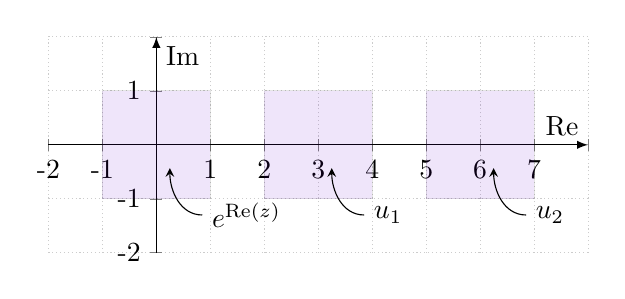
\begin{tikzpicture}
\begin{axis}[
  axis lines=middle,
  axis equal image,
  axis line style = {-latex},
  xmin=-2,xmax=8,ymin=-2,ymax=2,
  xtick distance = 1,
  ytick distance= 1,
  xticklabels = {\empty, -2, -1,0, 1,2,3,4,5,6,7,\empty},
  yticklabels = {\empty, -2 , -1, 0 , 1 , \empty},
  xlabel=Re,
  ylabel=Im,
  grid=major,
  grid style={thin,densely dotted,black!20}]
  \definecolor{mycolor}{RGB}{102,0,204}
 \draw[fill = mycolor, opacity = 0.1](axis cs:-1,-1) rectangle (axis cs: 1, 1) ;
 \draw[fill = mycolor, opacity = 0.1](axis cs: 2,-1) rectangle (axis cs: 4, 1) ;
  \draw[fill = mycolor, opacity = 0.1](axis cs: 5,-1) rectangle (axis cs: 7, 1) ;
  
  \node[anchor=west] (source1) at (axis cs:0.85, -1.3){ $e^{\mathrm{Re}(z)}$};
  \node (destination1) at (axis cs:0.25, -0.25){};
  \draw[->,>=stealth](source1) to [out=180,in=-90] (destination1);
  
  \node[anchor=west] (source2) at (axis cs:3.85, -1.3){ $u_1$};
  \node (destination2) at (axis cs:3.25, -0.25){};
  \draw[->,>=stealth](source2) to [out=180,in=-90] (destination2);
  
    \node[anchor=west] (source3) at (axis cs:6.85, -1.3){ $u_2$};
  \node (destination3) at (axis cs:6.25, -0.25){};
  \draw[->,>=stealth](source3) to [out=180,in=-90] (destination3);
\end{axis}
\end{tikzpicture}
\caption{Illustration of the construction of the activation function in \Cref{main_4}.}
\label{fig:illus}
\end{figure}

The preceding theorem showed that there exists an activation function for which the rate
in \Cref{main_2} can be strictly improved,
if one allows a discontinuous weight selection.
In contrast, the following theorem shows for a certain (quite natural) activation function
that the rate $m^{-k/(2n)}$ \emph{cannot} be improved (up to logarithmic factors),
even if one allows a discontinuous weight assignment.

\begin{theorem}\label{main_5}
   Let $n,k \in \NN$ and
  \begin{equation*}
    \phi: \quad \CC \to \CC, \quad \phi(z) \defeq \frac{1}{1+e^{-\mathrm{Re}(z)}}.
  \end{equation*}
  Then $\phi$ is smooth but non-polyharmonic.
  Furthermore, there exists a constant $c = c(n,k) > 0$ with the following property:
  For any $m \in \NN_{\geq 2}$ there exists a function $f \in C^k \left(\Omega_n ; \CC\right)$
  with $\Vert f \Vert_{C^k (\Omega_n; \CC)} \leq 1$, such that for every $\Phi \in \mathcal{F}^\phi_{n,m}$ and $\sigma \in \CC^m$ we have
  \begin{equation*}
      \left\Vert f - \sigma^T \Phi\right\Vert_{L^\infty \left(\Omega_n ; \CC\right)}
      \geq c \cdot \left(m \cdot \ln (m)\right)^{-k/(2n)}.
  \end{equation*}
\end{theorem}

\begin{proof}[Sketch of proof]
The idea of the proof is based on that of \cite[Theorem 4]{yarotsky_error_2017}
but instead of the bound for the VC dimension of ReLU networks used in \cite{yarotsky_error_2017},
we will employ a bound for the VC dimension stated in \cite[Theorem 8.11]{anthony_neural_1999}
using the real sigmoid function.
For a detailed introduction to the concept of the VC dimension and related topics,
see for instance \cite[Chapter 6]{shalev-shwartz_understanding_2014}.

A technical reduction from the complex to the real case (see \Cref{sec:main_5_reordered})
shows that it suffices to show the following:
If $\varepsilon \in (0,\frac{1}{2})$ and $m \in \NN$ are such that
for every $f \in C^k \left([-1,1]^n ; \RR\right)$ with $\left\Vert f \right\Vert_{C^k\left([-1,1]^n; \RR\right)} \leq 1$
there exists a real-valued shallow network $\mathcal{N}$ with $\gamma(x) = \frac{1}{1+e^{-x}}$
as activation function satisfying $\Vert f - \mathcal{N}\Vert_{L^\infty \left([-1,1]^n ; \RR\right)} \leq \varepsilon$,
then necessarily
\begin{equation*}
  m \geq c \cdot \frac{\varepsilon^{-n/k}}{  \mathrm{ln}\left( 1/\varepsilon\right)},
\end{equation*}
where the constant $c$ only depends on $n$ and $k$.

To show that the latter claim holds, we assume that $\varepsilon$ and $m$ have the property stated above.
Take $N \in \NN$ such that $N^{-k} \asymp \varepsilon$ and consider the grid 
\begin{equation*}
  \mathcal{G} \defeq \frac{1}{N} \{-N, ..., N\}^n \subseteq [-1,1]^n.
\end{equation*}
For every $\alpha \in \mathcal{G}$ we pick a number $z_\alpha \in \{0,1\}$ arbitrarily
and construct a map $f \in C^\infty ([-1,1]^n ; \RR)$ satisfying $f(\alpha) = z_\alpha$
for very $\alpha \in \mathcal{G}$.
Scaling of $f$ to $\tilde{f}$ ensures $\Vert \tilde{f} \Vert_{C^k ([-1,1]^n ; \RR)} \leq 1$,
but then $\tilde{f}(\alpha) = c_0 \cdot z_\alpha \cdot N^{-k}$ where $c_0 = c_0(n,k)>0$.
By assumption, we can infer the existence of a shallow real-valued neural network $\mathcal{N}$
with $\gamma$ as activation function and $m$ hidden neurons satisfying
$\Vert \tilde{f} - \mathcal{N} \Vert_{L^\infty([-1,1]^n ; \RR)} \leq \varepsilon$.
But this shows
\begin{equation*}
  \mathcal{N}(\alpha)
  \begin{cases}
    > \tilde{c} N^{-k}, & \mathrm{if} \ z_\alpha = 1, \\
    < \tilde{c} N^{-k}, & \mathrm{if} \ z_\alpha = 0
  \end{cases}
  \quad \text{for all } \alpha \in \mathcal{G}
\end{equation*}
with a constant $\tilde{c} = \tilde{c}(n,k)> 0$.
Since the $z_\alpha$ are arbitrary, it follows that the set
\begin{equation*}
  H
  \defeq \left\{
           \fres{\mathbbm{1}(\mathcal{N} > \tilde{c} N^{-k})}{\mathcal{G}}
           :
           \ \mathcal{N} \text{ shallow NN with activation $\gamma$ and $m$ hidden neurons}
         \right\}
\end{equation*}
\emph{shatters} the whole grid $\mathcal{G}$.
This yields $\mathrm{VC}(H) \geq \vert \mathcal{G} \vert = (2N + 1)^n$.
On the other hand, the bound provided by \cite[Theorem 8.11]{anthony_neural_1999}
for linear threshold networks yields $\mathrm{VC}(H) \lesssim m \cdot \ln(N)$.
Combining the two bounds and using $N^{-k} \asymp \varepsilon$ yields the claim.
\end{proof}

\section{Tractability of the considered problem in terms of the input dimension}\label{sec:cursetrac}

In this section we discuss the \emph{tractability} (in terms of the input dimension $n$)
of the considered problem, i.e., the dependence of the approximation error on $n$.
We show a novel result stating that, assuming a continuous weight selection,
the problem of approximating $C^k$-functions is \emph{intractable},
i.e., that the number of neurons that is required to achieve a non-trivial approximation error
is necessarily exponential in $n$.
In the literature this is referred to as the \emph{curse of dimensionality}.
The proof of the theorem combines ideas from \cite{devore_optimal_1989} and \cite{NOVAK2009398}
and is contained in \Cref{sec:intrac_reordered}.

\begin{theorem}\label{thm:intrac}
Let $s \in \NN$.
With $\Vert \cdot \Vert_{C^k([-1,1]^s;\RR)}$ defined similarly to \eqref{eq:ckdef}, we write
\begin{equation*}
  \Vert f \Vert_{C^\infty([-1,1]^s ; \RR)}
  \defeq \underset{k \in \NN}{\sup} \ \Vert f \Vert_{C^k([-1,1]^s; \RR)} \in [0, \infty]
\end{equation*}
for any function $f \in C^\infty([-1,1]^s ; \RR)$
and denote by $C^{\infty,\ast,s}$ the set of all $f \in C^\infty([-1,1]^s;\RR)$ for which this expression is finite. 
Let $\overline{a}: C^{\infty, \ast, s}\to \RR^{2^s - 1}$ be continuous with respect to some norm
on $C^{\infty, \ast, s}$ and moreover, let $M: \RR^{2^s - 1} \to C([-1,1]^s; \RR)$ be an arbitrary map.
Then it holds
\begin{equation*}
  \underset{\Vert f \Vert_{C^{\infty}([-1,1]^s;\RR)} \leq 1}{\underset{f \in C^{\infty, \ast,s}}{\sup}}
    \Vert f - M(\overline{a}(f))\Vert_{L^\infty([-1,1]^s ; \RR)}
  \geq 1.
\end{equation*}
\end{theorem} 
Note that \Cref{thm:intrac} is formulated for real-valued functions but can be transferred
to the complex-valued setting (see \Cref{corr:intrac_complex}).
We decided to include the real-valued statement because it is expected to be of greater interest
in the community than the complex-valued analog.
Moreover, we stress that \Cref{thm:intrac} is not limited to the class of shallow neural networks
but refers to any function class that is parametrizable using finitely many parameters
(in particular, e.g., the class of neural networks with possibly more than one hidden layer).

We now examine in what way the constant $c$ appearing in \Cref{main_2} suffers from the curse of dimensionality.
To this end, it is convenient to rewrite the result from \Cref{main_2} as
\begin{equation*}
  \sup_{\Vert f \Vert_{C^k(\Omega_n; \CC)} \leq 1} \ \ \underset{}{\inf_{\Phi \in \mathcal{F}^\phi_{n,m},\sigma \in \CC^m}}
    \Vert f - \sigma^T \Phi \Vert_{L^\infty(\Omega_n ; \CC)}
  \leq \left(\tilde{c} \cdot m\right)^{-k/(2n)}
\end{equation*}
where the constant $\tilde{c} = \tilde{c}(n,k)> 0$ is independent of $m$.
Writing the result in that way, one sees immediately that, if one seeks to have a worst-case approximation error
of less than $\varepsilon>0$, it is sufficient to take $m = \left\lceil\frac{1}{\tilde{c}} \cdot \varepsilon^{-(2n)/k} \right\rceil$
neurons in the hidden layer of the network.
\Cref{corr:const_intrac} shows that it \emph{necessarily} holds $\tilde{c} \leq 16 \cdot  2^{-n}$ and therefore,
the constant $\tilde{c}$ unavoidably suffers from the curse of dimensionality.
An analysis of the constant
(where we refer to \Cref{ck_functions_reordered,sec:const_bound_reordered,sec:fourier_reordered} for the details)
shows that in our case we can establish the bound $\tilde{c}(n,k) \geq \exp(-C \cdot n^2) \cdot k^{-4n}$
with an \emph{absolute} constant $C>0$.
We remark that, since the constant suffers from the curse of dimensionality in any case,
we have not put much effort into optimizing the constant; there is therefore probably ample room for improvement.


\section{Limitations}

To conduct a comprehensive evaluation of machine learning algorithms,
one must analyze the questions of approximation, generalization, and optimization through training algorithms.
The present paper, however, only focuses on the aspect of approximation.
Analyzing if the proven approximation rate can be attained with learning algorithms
such as (stochastic) gradient descent falls outside the scope of this paper.
Furthermore, the examination of approximation rates under possibly discontinuous weight assignment
is not yet fully resolved by our results.
It is an open question which rate is optimally achievable in that case,
depending on the choice of the activation function, and specifically in distinguishing
between shallow and deep networks. We want to mention the two following points
which indicate that this is a quite subtle question:
\begin{enumerate}
\item For deep NNs (with more than two hidden layers) with general smooth activation function,
      it is \emph{not possible} to derive any non-trivial lower bounds in the setting of unrestricted weight assignment,
      since there exists an activation function with the property that NNs of \emph{constant size}
      using this activation function can approximate any continuous function to arbitrary precision
      (see \cite[Theorem 4]{MAIOROV199981}).
      Note that \cite{MAIOROV199981} considers real-valued NNs, but the results can be transferred to CVNNs
      with a suitable choice of the activation function.

\item In the real-valued case, fully general lower bounds for the approximation capabilities of shallow NNs
      have been derived by using results from \cite{gordon_best_2001}
      regarding the approximation properties of so-called ridge functions,
      i.e., functions of the form $\sum_{j=1}^m \phi_j(\langle a_j, x \rangle)$
      with $a_j \in \RR^d$ and each $\phi_j: \RR \to \RR$.
      It is an interesting problem to generalize these results to higher-dimensional ridge functions
      of the form $\sum_{j=1}^m \phi_j(A_j x)$, where each $\phi_j: \RR^s \to \RR$ and $A_j \in \RR^{s \times d}$.
      This would imply lower bounds for shallow CVNNs.
      However, such a generalization seems to be highly non-trivial and is outside the scope of the present paper.
\end{enumerate}


\section{Conclusion}

This paper analyzes error bounds for the approximation of complex-valued $C^k$-functions
by means of complex-valued neural networks with smooth and non-polyharmonic activation functions.
It is demonstrated that complex-valued neural networks with these activation functions
achieve the \emph{identical} approximation rate as real-valued networks that employ
smooth and non-polynomial activation functions.
This is an important theoretical finding, since CVNNs are on the one hand more restrictive
than real-valued neural networks (since the mappings between layers should be $\CC$-linear
and not just $\RR$-linear), but on the other hand more versatile,
since the activation function is a mapping from $\CC$ to $\CC$
(i.e., from $\RR^2 \to \RR^2$) rather than from $\RR$ to $\RR$ as in the real case.
Additionally, it is established that the proven approximation rate is optimal if one assumes
a continuous weight selection.
In summary, if one focuses on the approximation rate for $C^k$-functions,
CVNNs have the same excellent approximation properties as real-valued networks.

The behavior of the approximation rate for unrestricted weight selection is more subtle.
It is shown that a rate of $m^{-k/(2n-1)}$ can be achieved for certain activation functions (\Cref{main_4})
but in general, one cannot improve on the rate that is attainable for continuous weight selection (\Cref{main_5}).   

While the proven approximation \emph{rate} is optimal under the assumption of continuous weight selection,
the involved constants suffer from the curse of dimensionality.
\Cref{sec:cursetrac}, however, shows that this is inevitable in the given setting. 

Such theoretical approximation results contribute to the mathematical understanding of Deep Learning.
The remarkable approximation-theoretical properties of neural networks can be seen as one reason
why neural networks provide outstanding results in many applications.

\newpage

\textbf{Acknowledgments.}
PG and FV acknowledge support by
the German Science Foundation (DFG) in the context of the Emmy Noether junior research
group VO 2594/1-1. FV acknowledges support by the Hightech Agenda Bavaria. 

\printbibliography

\appendix
\section{Appendix for Proofs}

\paragraph{Proof of Theorem \ref{thm:main}.}

\begin{proof}
\label{proof:main}
Our proof has two steps. In Step 1, we will show that SimCLR is equivalent to minimizing the cross entropy loss defined in Eqn.~(\ref{eqn:cross-entropy}). 
In Step 2, we will show  that minimizing the cross-entropy loss 
is equivalent to spectral clustering on $\bfpi$. 
Combining the two steps together, we have proved our theorem. 

\textbf{Step 1: } SimCLR is equivalent to minimizing the cross entropy loss.

The cross-entropy loss takes expectation over 
$\bfW_\bfX\sim \mathbb{P}(\cdot ; \bfpi)$, 
which means $\bfW_\bfX$ has exactly one non-zero entry in each row $i$. By Lemma~\ref{lem:multinomial}, we know every row $i$ of $\bfW_\bfX$ is independent of other rows. Moreover, 
$\bfW_{\bfX,i}\sim \mathcal{M}(1, \bfpi_i/\sum_j \bfpi_{i,j})=\mathcal{M}(1, \bfpi_i)$, because $\bfpi_i$ itself is a probability distribution.
Similarly, we know $\bfW_\bfZ$ also has the row-independent property by sampling over $\mathbb{P}(\cdot;\bfK_\bfZ)$.
Therefore, by Lemma~\ref{lem:cross_split}, we know Eqn.~(\ref{eqn:cross-entropy}) is equivalent to:
\[
 -\sum_{i=1}^n \mathbb{E}_{\bfW_{\bfX,i}}[\log \mathbb{P}(\bfW_{\bfZ,i}=\bfW_{\bfX,i};\bfK_\bfZ)],
\]

This expression takes expectation over $\bfW_{\bfX,i}$ for the given row $i$. Notice that 
$\bfW_{\bfX,i}$ has exactly one non-zero entry, which equals $1$ (same for $\bfW_{\bfZ,i}$). 
As a result
we expand the above expression to be:
\begin{equation}
 -\sum_{i=1}^n \sum_{j\neq i} \Pr(\bfW_{\bfX,i,j}=1)\log \Pr(\bfW_{\bfZ,i,j}=1).
\label{eqn:detailed-expansion}    
\end{equation}


By Lemma~\ref{lem:multinomial}, $\Pr(\bfW_{\bfZ,i,j}=1)=\bfK_{\bfZ,i,j}/\|\bfK_{\bfZ,i}\|_1$ for $j\neq i$. Recall that $\bfK_\bfZ=(k(\bfZ_i-\bfZ_j))_{(i,j)\in[n]^2}$, which means 
$\bfK_{\bfZ,i,j}/\|\bfK_{\bfZ,i}\|_1=\frac{\exp(-\|\bfZ_i-\bfZ_j\|^2/{2\tau})}{\sum_{k\neq i}
\exp(-\|\bfZ_i-\bfZ_k\|^2/{2\tau})
}$ for $j\neq i$, when $k$ is the Gaussian kernel with variance $\tau$. 

Notice that $\bfZ_i=f(\bfX_i)$, so we know
\begin{equation}
-\log \Pr(\bfW_{\bfZ,i,j}=1)=
-\log \frac{\exp(-\|f(\bfX_i)-f(\bfX_j)\|^2/{2\tau})}{\sum_{k\neq i}
\exp(-\|f(\bfX_i)-f(\bfX_k)\|^2/{2\tau}),
}
\label{eqn:infonce-equivalence}    
\end{equation}


The right hand side is exactly the InfoNCE loss defined in Eqn.~(\ref{eqn:infonce}).
Inserting Eqn.~(\ref{eqn:infonce-equivalence}) into Eqn.~(\ref{eqn:detailed-expansion}), we get the SimCLR algorithm, which first samples augmentation pairs $(i,j)$ with $\Pr(\bfW_{\bfX,i,j}=1)$ for each row $i$, and then optimize the InfoNCE loss. 

\textbf{Step 2: } minimizing the cross entropy loss 
is equivalent to spectral clustering on $\bfpi$.


By Lemma~\ref{lem:convert_to_spectral}, we may further convert the loss to 
\begin{equation}
\label{eqn:main-theorem-repul-attr}
\min_{\bfZ}
-\sum_{(i,j)\in [n]^2} \mathbf{P}_{i,j}
\log k (\bfZ_i-\bfZ_j)+\log \mathbf{R}(\bfZ).
\end{equation}
Since $k$ is the Gaussian kernel, this reduces to \[
\min_\bfZ \mathrm{tr}(\bfZ^\top \mathbf{L}(\bfpi) \bfZ)
+\log \mathbf{R}(\bfZ),
\]

where we use the fact that $\mathbb{E}_{\bfW_\bfX\sim \mathbb{P}(\cdot; \bfpi)}[\mathbf{L}(\bfW_\bfX)]
=\mathbf{L}(\bfpi)
$, because the Laplacian operator is linear and $
\mathbb{E}_{\bfW_\bfX\sim \mathbb{P}(\cdot; \bfpi)}(\bfW_\bfX)=\bfpi
$.
\end{proof}

\paragraph{Proof of Theorem \ref{thm:clip}.}
\begin{proof}
Since $\bfW_\bfX\sim \mathbb{P}(\cdot;\bfpi_{\mathbf{A}, \mathbf{B}})$, we know 
$\bfW_\bfX$ has exactly one non-zero entry in each row, denoting the pair that got sampled. 
A notable difference compared to the previous proof is we now have $n_\mathcal{A}+n_\mathcal{B}$ objects in our graph. CLIP deals with this by taking a mini-batch of size $2N$, 
such that $n_\mathcal{A}=n_\mathcal{B}=N$, and adding the $2N$ InfoNCE losses together. We label the objects in $\mathcal{A}$ as $[n_\mathcal{A}]$, and the objects in $\mathcal{B}$ as $\{n_\mathcal{A}+1, \cdots, n_\mathcal{A}+n_\mathcal{B}\}$. 

Notice that $\bfpi_{\mathbf{A}, \mathbf{B}}$ is a bipartite graph, so the edges of objects in $\mathcal{A}$ will only connect to object in $\mathcal{B}$ and vice versa. We can define the similarity matrix in $\cZ$ as $\bfK_\bfZ$, 
where $\bfK_\bfZ(i, j+n_\mathcal{A})=\bfK_\bfZ(j+n_\mathcal{A},i)= k(\bfZ_i-\bfZ_j)$ for $i\in [n_\mathcal{A}], j\in [n_\mathcal{B}]$, and otherwise we set $\bfK_\bfZ(i,j)=0$. 
The rest is same as the previous proof. 
\end{proof}

\paragraph{Proof of Theorem \ref{thm:exponential}.}

\begin{proof}
\label{proof:exponential}
Since the objective function consists of a linear term combined with an entropy regularization, which is a strongly concave function, the maximization problem is a convex optimization problem. Owing to the implicit constraints provided by the entropy function, the problem is equivalent to having only the equality constraint. We then introduce the Lagrangian multiplier $\lambda$ and obtain the following relaxed problem:

$$
\widetilde{E}(\boldsymbol{\alpha})=\psi_{1}-\sum_{i=1}^n \alpha_{i} \psi_{i}+\tau \sum_{i=1}^n \alpha_{i}\log \alpha_{i}+\lambda\left(\boldsymbol{\alpha}^{\top} \mathbf{1}_n-1\right).
$$

As the relaxed problem is unconstrained, taking the derivative with respect to $\alpha_{i}$ yields

$$
\frac{\partial \widetilde{E}(\boldsymbol{\alpha})}{\partial \alpha_{i}}=-\psi_{i}+\tau\left(\log \alpha_{i}+\alpha_{i} \frac{1}{\alpha_{i}}\right)+\lambda=0.
$$

Solving the above equation implies that $\alpha_{i}$ takes the form
$
\alpha_{i}=\exp \left(\frac{1}{\tau} \psi_{i}\right) \exp \left(\frac{-\lambda}{\tau}-1\right).
$ Since $\alpha_{i}$ lies on the probability simplex, the optimal $\alpha_{i}$ is explicitly given by
$
\alpha^{*}_{i}=\frac{\exp \left(\frac{1}{\tau} \psi_{i}\right)}{\sum_{i^{\prime}=1}^n \exp \left(\frac{1}{\tau} \psi_{i^{\prime}}\right)} .
$ Substituting the optimal point into the objective function, we obtain
$$
\begin{aligned}
E\left(\boldsymbol{\alpha}^*\right)  &=\psi_1-\sum_{i=1}^n \frac{\exp \left(\frac{1}{\tau} \psi_{i}\right)}{\sum_{i^{\prime}=1}^n \exp \left(\frac{1}{\tau} \psi_{i^{\prime}}\right)} \psi_{i}+\tau \sum_{i=1}^n \frac{\exp \left(\frac{1}{\tau} \psi_{i}\right)}{\sum_{i^{\prime}=1}^n \exp \left(\frac{1}{\tau} \psi_{i^{\prime}}\right)}\log \frac{\exp \left(\frac{1}{\tau} \psi_{i}\right)}{\sum_{i^{\prime}=1}^n \exp \left(\frac{1}{\tau} \psi_{i^{\prime}}\right)} \\
& =\psi_1 - \tau \log \left(\sum_{i=1}^n \exp \left(\frac{1}{\tau} \psi_{i}\right)\right).
\end{aligned}
$$
Thus, the Lagrangian dual function is given by
\begin{equation*}
-E\left(\boldsymbol{\alpha}^*\right)= -\tau \log \frac{\exp \left(\frac{1}{\tau} \psi_{1}\right)}{\sum_{i=1}^n \exp \left(\frac{1}{\tau} \psi_{i}\right)}.\qedhere
\end{equation*}
\end{proof}



\section{More on Experiments} \label{section: experiment_details}

\paragraph{CIFAR-10 and CIFAR-100} CIFAR-10 ~\citep{krizhevsky2009learning} and CIFAR-100 ~\citep{krizhevsky2009learning} are well-known classic image classification datasets. Both CIFAR-10 and CIFAR-100 contain a total of 60k $32 \times 32$ labeled images of different classes, with 50k for training and 10k for testing. CIFAR-10 is similar to CIFAR-100, except there are 10 different classes in CIFAR-10 and 100 classes in CIFAR-100.

\paragraph{TinyImageNet} TinyImageNet ~\citep{le2015tiny} is a subset of ImageNet ~\citep{deng2009imagenet}. There are 200 different object classes in TinyImageNet, with 500 training images, 50 validation images, and 50 test images for each class. All the images in TinyImageNet are colored and labeled with a size of $64 \times 64$.

\textbf{Pseudo-code.} Algorithm \ref{alg:Training Procedure} presents the pseudo-code for our empirical training procedure.

\begin{algorithm}[!htbp]
\caption{Training Procedure}
\label{alg:Training Procedure}
\begin{algorithmic}[1]
\REQUIRE trainable encoder network $f$, batch size $N$, augmentation strategy \textit{aug}, loss function $L$ with hyperparameters \textit{args}
\FOR {sampled minibatch ${x_i}_{i=1}^N$}
\FORALL{$i \in { 1, ..., N }$}
\STATE draw two augmentations $t_i = \textit{aug}\left(x_i\right) $, $t_i' = \textit{aug}\left(x_i\right) $
\STATE $z_i = f\left(t_i\right)$, $z_i' = f\left(t_i'\right)$
\ENDFOR
\STATE compute loss $\mathcal{L} = L(N, z, z', \textit{args})$
\STATE update encoder network $f$ to minimize $\mathcal{L}$
\ENDFOR
\STATE \textbf{Return} encoder network $f$
\end{algorithmic}
\end{algorithm}

We also provide the pseudo-code for our core loss function used in the training procedure in Algorithm \ref{alg:Core loss}. The pseudo-code is almost identical to SimCLR's loss function, with the exception of an extra parameter $\gamma$.

\begin{algorithm}[!htbp]
\caption{Core loss function $\mathcal{C}$}
\label{alg:Core loss}
\begin{algorithmic}[1]
\REQUIRE batch size $N$, two encoded minibatches $z_1, z_2$, $\gamma$, temperature $\tau$
\STATE $z = \textit{concat}\left(z_1, z_2\right)$
\FOR {$i \in {1, ..., 2N }, j \in {1, ..., 2N}$ }
\STATE $s_{i,j} = \Vert z_i - z_j \Vert_2^{\gamma}$
\ENDFOR
\STATE \textbf{define} $l(i, j)$ \textbf{as} $l(i, j) = - \log \frac{exp\left(s_{i,j}/\tau \right)}{\sum_{k=1}^{2N} \mathbf{1}{[k \ne i]} exp\left(s{i, j} / \tau \right)} $
\STATE \textbf{Return} $\frac{1}{2N} \sum_{k=1}^N\left[l(i, i+N) + l(i+N, i)\right]$
\end{algorithmic}
\end{algorithm}

Utilizing the core loss function $\mathcal{C}$, we can define all kernel loss functions used in our experiments in Table \ref{table: loss definition}. For all $z_i \in z$ with even dimensions $n$, we define $z_{L_i} = z_i\left[0:n/2\right]$ and $z_{R_i} = z_i\left[n/2:n\right]$.

\begin{table}[ht]
\centering
\begin{tabular}{{@{}l|l@{}}}
Kernel  &  Loss function \\ \midrule
Laplacian & $\mathcal{C}\left(N, z, z', \gamma=1, \tau\right)$\\ \midrule
Sum       & $\lambda * \mathcal{C}\left(N, z, z', \gamma=1, \tau_1\right) + (1-\lambda) * \mathcal{C}\left(N, z, z', \gamma=2, \tau_2\right)$  \\ \midrule
Concatenation Sum&$\lambda * \mathcal{C}\left(N, z_L, z'_L, \gamma=1, \tau_1\right) + (1-\lambda) * \mathcal{C}\left(N, z_R, z'_R, \gamma=2, \tau_2\right)$\\ \midrule
$\gamma = 0.5$ & $\mathcal{C}\left(N, z, z', \gamma=0.5, \tau\right)$          \\ 

\end{tabular}

\caption{Definition of kernel loss functions in our experiments}
\label {table: loss definition}
\end{table}

\textbf{Baselines.} We reproduce the SimCLR algorithm using PyTorch Lightning~\citep{PytorchLightning}.

\textbf{Encoder details.}
The encoder $f$ consists of a backbone network and a projection network. We employ ResNet50~\citep{ResNet} as the backbone and a 2-layer MLP (connected by a batch normalization~\citep{ioffe2015batch} layer and a ReLU \cite{nair2010rectified} layer) with hidden dimensions 2048 and output dimensions 128 (or 256 in the concatenation kernel case).

\textbf{Encoder hyperparameter tuning.}
For each encoder training case, we randomly sample 500 hyperparameter groups (sample details are shown in Table \ref{table: Hyperparameter sample}) and train these samples simultaneously using Ray Tune ~\citep{RayTune}, with the ASHA scheduler~\citep{li2018massively}. Ultimately, the hyperparameter group that maximizes the online validation accuracy (integrated in PyTorch Lightning) within 5000 validation steps is chosen for the given encoder training case.

\begin{table}[ht]
\centering

\begin{tabular}{@{}l|l|l@{}}
\midrule
Hyperparameter  & Sample Range & Sample Strategy \\ \midrule
start learning rate & $\left[10^{-2}, 10\right]$ & log uniform \\ \midrule
$\lambda$       & $\left[0, 1\right]$ & uniform \\ \midrule
$\tau$, $\tau_1$, $\tau_2$ & $\left[0, 1\right]$ & log uniform \\ \midrule
\end{tabular}

\caption{Hyperparameters sample strategy}
\label {table: Hyperparameter sample}
\end{table}

\textbf{Encoder training.} 
We train each encoder using the LARS optimizer~\citep{LARSOptimizer}, LambdaLR Scheduler in PyTorch, momentum 0.9, weight decay $10^{-6}$, batch size 256, and the aforementioned hyperparameters for 400 epochs on a single A-100 GPU.

\textbf{Image transformation.} The image transformation strategy, including augmentation, is identical to the default transformation strategy provided by PyTorch Lightning.

\textbf{Linear evaluation.}
The linear head is trained using the SGD optimizer with a cosine learning rate scheduler, batch size 64, and weight decay $10^{-6}$ for 100 epochs. The learning rate starts at $0.3$ and ends at $0$.

\textbf{Moco Experiments.} We also tested our method based on MoCo~\citep{he2019moco}. The results are summarized in Table \ref{tab:results-moco}. Here we choose ResNet18~\citep{ResNet} as the backbone and set a temperature of $0.1$ as default. For our simple sum kernel, we set $\lambda=0.8$. The results show that our method outperforms the original MoCo method.

\begin{table}[thb]
\centering
\caption{MoCo Experiment Results on CIFAR-10 and CIFAR-100.}
\label{tab:results-moco}
\resizebox{\textwidth}{!}{%
\begin{tabular}{@{}c|ccc|ccc@{}}
\toprule
\multirow{3}{*}{Method} & \multicolumn{3}{c|}{CIFAR-10} & \multicolumn{3}{c}{CIFAR-100} \\ \cmidrule(lr){2-4} \cmidrule(lr){5-7} 
                        & 200 epochs & 400 epochs    & 1000 epochs   & 200 epochs & 400 epochs & 1000 epochs         \\ \midrule
MoCo (repro.)         & $76.41 \pm 0.12$    & $80.01 \pm 0.15$          & $84.45 \pm 0.08$    & $\mathbf{47.02 \pm 0.11}$ & $52.50 \pm 0.07$ & $57.62 \pm 0.15$            \\
\midrule
Laplacian Kernel        & ${78.09 \pm 0.10}$    & $\mathbf{83.85 \pm 0.09}$          & $\mathbf{88.34 \pm 0.16}$    & $46.12 \pm 0.22$   & $53.44 \pm 0.17$ & $59.10 \pm 0.14$        \\
Simple Sum Kernel & $\mathbf{78.12 \pm 0.15}$   & $83.23 \pm 0.18$ & $87.50 \pm 0.20$ & $46.65 \pm 0.06$ & $\mathbf{53.62 \pm 0.19}$ & $\mathbf{59.83 \pm 0.12}$\\
\bottomrule
\end{tabular}
}
\end{table}



\section{More Experiments on Synthetic Data}


Consider a scenario with $n$ clusters, each containing $k$ vertices. Let the probability of vertices $u$ and $v$ from the same cluster belonging to $\bfpi$ be $p$. Conversely, for vertices $u$ and $v$ from different clusters, let the probability of belonging to $\pi$ be $q$. We generate the graph $\bfpi$ randomly, based on $p$ and $q$. We experiment with values of $k=100$ and $n=6$ for ease of visualization, embedding all points in a two-dimensional space. Each vertex's initial position originates from a normal distribution. In each iteration, we sample a subgraph of $\bfpi$ uniformly, ensuring each vertex has an out-degree of $1$. We then optimize the corresponding vectors using InfoNCE loss with an SGD optimizer and iterate until convergence. Our experimental setup consists of an SGD learning rate of $1$, an InfoNCE loss temperature of $0.5$, and a batch size of $50$. We evaluate two scenarios with different $p$ and $q$ values: $p=1$, $q=0$, and $p=0.75$, $q=0.2$. The results of these experiments are visualized in Figure \ref{fig:vis-spectral-cluster}. The obtained embeddings exhibit the hallmark pattern of spectral clustering of graph $\bfpi$.

\begin{figure}[!tb]
\centering
\subfigure{
\includegraphics[width=1\textwidth]{Figures/cluster_pi.png}
\label{fig:vis-cluster}
}
\subfigure{
\includegraphics[width=1\textwidth]{Figures/noised_cluster_pi.png}
\label{fig:vis-noised-cluster}
}
\caption{Visualizations of the optimization process using InfoNCE Loss on the vectors corresponding to $\bfpi$. Points of identical color belong to the same cluster within $\bfpi$. To showcase the internal structure of $\bfpi$, we randomly select 10 vertices from each cluster to display the edge distribution of $\bfpi$.}
\label{fig:vis-spectral-cluster}
\end{figure}








\end{document}
